\documentclass[prd,preprintnumbers,twocolumn,eqsecnum,floatfix,a4paper,nofootinbib,superscriptaddress]{revtex4}
\usepackage{color}
\usepackage{calc}
\usepackage{amsmath,amssymb,graphicx}
\usepackage{amssymb,amsmath}
\usepackage{bm}
\usepackage{microtype}
\usepackage{booktabs}
\usepackage{times}
\usepackage[varg]{txfonts}
\usepackage[colorlinks, pdfborder={0 0 0}]{hyperref}
\usepackage[utf8]{inputenc}
\definecolor{LinkColor}{rgb}{0.75, 0, 0}
\definecolor{CiteColor}{rgb}{0, 0.5, 0.5}
\definecolor{UrlColor}{rgb}{0, 0, 0.75}
\hypersetup{linkcolor=LinkColor}
\hypersetup{citecolor=CiteColor}
\hypersetup{urlcolor=UrlColor}
\maxdeadcycles=1000
\allowdisplaybreaks
\textwidth 7 in
\hoffset -0.1in
\textheight 10in
\DeclareFontFamily{OT1}{pzc}{}
\DeclareFontShape{OT1}{pzc}{m}{it}{<-> s * [1.10] pzcmi7t}{}
\DeclareMathAlphabet{\mathpzc}{OT1}{pzc}{m}{it}
\newcommand{\comment}[1]{\textcolor{blue}{\textit{#1}}}
\newcommand{\ajith}[1]{\textcolor{red}{\textit{Ajith:#1}}}
\newcommand{\checkthis}{\textcolor{magenta}{(CHECKTHIS)}}
\newcommand{\vijay}[1]{\textcolor{cyan}{Vijay: #1}}
\newcommand{\io}{\iota}
\newcommand{\p}{\phi}
\newcommand{\vp}{\varphi}

\newcommand{\h}{\mathpzc{h}}
\newcommand{\Hhat}{\hat{\mathpzc{H}}}
\newcommand{\B}{\mathpzc{B}}
\newcommand{\hlm}{\mathpzc{h}_{\ell m}}
\newcommand{\xilm}{\xi_{\ell m}}
\newcommand{\Ylm}{{Y}^{-2}_{\ell m}}
\newcommand{\Y}{{Y}^{-2}}
\newcommand{\hc}{h_\times}
\newcommand{\hp}{h_+}
\newcommand{\Fc}{F_\times}
\newcommand{\Fp}{F_+}
\newcommand{\Mf}{M_f}
\newcommand{\cA}{\mathpzc{A}}
\newcommand{\lm}{_{\ell m}}
\newcommand{\deff}{d_\mathrm{eff}}
\newcommand{\rmi}{\mathrm{i}}
\newcommand{\blambda}{\bm{\lambda}}
\newcommand{\btheta}{\bm{\theta}}
\newcommand{\Mo}{M_{\odot}}
\newcommand{\FFe}{\mathrm{FF}_\mathrm{eff}}
\newcommand{\FF}{\mathrm{FF}}
\newcommand{\e}{\mathrm{e}}
\newcommand{\rhoopt}{\rho_\mathrm{opt}}
\newcommand{\rhosubopt}{\rho_\mathrm{subopt}}
\newcommand{\fqnm}{f}
\newcommand{\sigmaqnm}{\sigma}

\newcommand*{\skymapscale}{0.5}
\newcommand*{\paramestscale}{0.455}

\begin{document}

\newcommand{\be}{\begin{equation}}
\newcommand{\ee}{\end{equation}}
\newcommand{\ber}{\begin{eqnarray}}
\newcommand{\eer}{\end{eqnarray}}
\def\bea{\begin{eqnarray}}
\def\eea{\end{eqnarray}}
\newcommand{\etal}{\emph{et al}}

\title{A consistency test of general relativity using different multipoles of \\gravitational radiation from binary black holes}
\author{Siddharth Dhanpal}
\affiliation{International Centre for Theoretical Sciences, Tata Institute of Fundamental Research, Bangalore 560012, India}
\author{Abhirup Ghosh}
\affiliation{International Centre for Theoretical Sciences, Tata Institute of Fundamental Research, Bangalore 560012, India}
\author{Parameswaran~Ajith}
\affiliation{International Centre for Theoretical Sciences, Tata Institute of Fundamental Research, Bangalore 560012, India}
\affiliation{Canadian Institute for Advanced Research, CIFAR Azrieli Global Scholar, MaRS Centre, West Tower, 661 University Ave., Suite 505, Toronto, ON M5G 1M1, Canada}
\author{B.~S.~Sathyaprakash}
\affiliation{Penn State University}

\begin{abstract}
\end{abstract}
\preprint{LIGO-}
\maketitle
%%%%%%%%%%%%%%%%%%%%%%%%%%%%%%%%%%%%%%%%%%%%%%%%%%%%%%%%%%%%%%%%%%%%%%%%%%%%%%%%%%%%%%%%%%%%%%%%%%%%%%%%%%%%%%%%%%%%%%%%%%%%%%%%%%%%%%%%%%%%%%%`
\paragraph{Introduction:---}

Recent observations of gravitational-wave (GW) signals from merging binaries of black holes~\cite{bbh_refs} and neutron stars~\cite{bns_ref} by LIGO~\cite{ligo_ref} and Virgo~\cite{virgo_ref} have enabled the first tests of General Relativity (GR) in the highly relativistic regime. 

\paragraph{Testing the consistency between different multipoles of the gravitational radiation:--}
An interferometric GW detector observes a linear combination of the two polarizations $h_+(t)$ and $h_\times(t)$ of the GW signal, given by 
\begin{equation}
h(t) = F_+(\theta, \phi, \psi) \, h_+(t-t_0) + F_{\times}(\theta, \phi, \psi), {h}_{\times}(t-t_0), 
\label{eq:det_response}
\end{equation}
where $F_+$ and $F_x$ are the antenna pattern functions of the GW detector, $t_0$ is the time of arrival of the signal at the detector, and $(\theta, \phi, \psi)$ define the sky position and polarisation of the GW source respectively. The two GW polarizations $\h := h_+(t) -i h_\times(t)$ can be expanded in a basis of spin $-2$ weighted spherical harmonics, as:
\begin{equation}
\h(t; \iota, \phi_0, \blambda) = \sum _{\ell=2}^{\infty} \sum _{m=-\ell}^{\ell} \Ylm (\iota, \phi_0) \, \frac{{\h}_{lm}(t; \blambda)}{d_L}, 
\label{eq:spherical_harmonics}
\end{equation}
where $\Ylm$ are the basis functions of spin $-2$ spherical harmonics, $(\iota, \phi_0)$ define the direction of radiation in the source frame, $d_L$ is  the luminosity distance to the binary, and 
${\h}_{lm}(t; \blambda)$ are the spherical harmonic modes of the waveform, which are completely described by the intrinsic parameters $\blambda := \{m_1, m_2\}$ of the system. We assume that the black holes are non-spinning and the binary to be qusi-circular. Hence $\blambda$ consists of only the masses $m_1$ and $m_2$ of the black holes. 

In GR, the set of intrinsic parameters $\blambda$ completely determines the multipolar structure of the waveform ${\h}_{lm}(t)$. Any inconsistency between the different multipoles of the radiation can point to a deviation from GR. In this paper, we propose a test of GR based on the consistency of different multipoles of the gravitational radiation from binary black holes. In order to formulate a consistency test between different multipoles, we rewrite Eq.(\ref{eq:spherical_harmonics}) by splitting the contributions from the dominant $(\ell = 2, m = \pm 2)$ mode of gravitational radiation, and the sub-dominant (higher order) modes 
\begin{eqnarray}
\h(t; \iota, \phi_0, \blambda) & = & \sum_{m = -2,2} Y^{-2}_{2m} (\iota, \phi_0) {\h}_{2m}(t, \blambda)  \nonumber \\ 
 & + & \sum _{\text{H.O.M}} \Ylm (\iota, \phi_0) \h_{lm}(t, \blambda+\Delta \blambda)
\label{eq:test_HM}
\end{eqnarray}
where the subscript H.O.M underneath the summation in the second term on the RHS indicates contribution from just the higher-order multipoles of the gravitational radiation. Note that we allow a possibility of inconsistency between the dominant mode and higher order modes by introducing a deviation $\Delta \blambda$ in the set of intrinsic parameters that describe the higher order modes; in GR,  $\Delta \blambda = 0$. 

The data $d(t)$ contains the observed signal $h(t)$ given in Eq.~(\ref{eq:det_response}) along with noise, which is well described by a stationary Gaussian random process 
\begin{equation}
d(t) = n(t) + h(t)
\label{eq:detector_strain}
\end{equation}
For coalescencing binary black hole (BBH) systems in quasi-circular orbits, the observed signal $h(t)$ is described by a set of 9 parameters $\btheta := \{m_1, m_2, t_0, \phi_0, d_L, \theta, \phi, \psi, \iota\}$ in GR. Given data $d$ and assuming a particular model of the waveform as our hypothesis $H$, it is possible to compute the posterior distribution of $\btheta$ making use of the Bayes theorem, which states: 
\begin{equation}
P(\btheta|d, H, I) = \frac{P(\btheta|H, I) \, \mathcal{L}(d|\btheta, H, I)}{Z(d|H, I)}
\label{eq:Bayes_theorem}
\end{equation} 
The first term of the numerator on the RHS, $P(\theta|H,I)$ is the \emph{prior} distribution of $\btheta$, the second term $\mathcal{L}(d|\btheta, H,I)$ is the \emph{likelihood} function, and the term in the denominator $E(d|H,I)$ is a normalisation constant, called the \emph{evidence}, and \emph{I} is any other information used in the analysis. For stationary Gaussian noise with power spectral density $S_n(f)$, the likelihiood can be written as:
\begin{equation}
\mathcal{L}({d}|\theta, H,I) = \text{exp}\Big[ -\frac{1}{2}\int_{f_\mathrm{low}}^{f_\mathrm{high}} \frac{|\tilde{d}(f) - \tilde{h}(f;\theta, H)|^2}{S_n(f)}df\Big]
\end{equation}
where $f_\mathrm{low}$ and $f_\mathrm{high}$ define the sensitivity bandwidth of the detector, while $\tilde{d}(f)$ and $\tilde{h}(f)$ are the Fourier transforms of $(d(t)$ and $h(t))$, respectively. 

Using the above definition for the likelihood function, one proceeds to estimate $\theta$ by stochastically sampling over the entire parameter space using  \emph{emcee}~\cite{goodman2010ensemble,foreman2013emcee}, an ensemble Markhov chain Monte Carlo sampler, which uses the underlying property of affine invariance of all Gaussian distributions to sample from highly skewed distributions a lot faster than standard single-particle methods, such as Metropolis-Hastings implementations. A MCMC scheme is a random walk through the parameter space $\theta$ generating samples of $\theta$ with a probability density which ultimately converges to the stationary distribution of the Markhov chain, the posterior PDF $p(\theta|d, H, I)$, using the equation of detailed balance. An \emph{ensemble} MCMC sampler implements a coordinated random walk of multiple "walkers" through the parameter space, such that each step of the Markhov chain, or updating the position of any one walker at a paricular time step, is influenced by the positions of the rest of the walkers. The specific move used by the sampler is called the \emph{stretch} move (described in detail in section 2. of ~\cite{goodman2010ensemble}). The algorithm requires the hand-tuning of a small set of 1-2 parameters, and can be easily parallelised to use multiple CPU cores, giving it major advantages over traditional MCMC algorithms.

\paragraph{Simulations and results:---}

%%%%%%%%%%%%%%%%%%%%%%%%%%%%%%%%%%%%%%%%%%%%%%%%%%%%%%%%%%%%%%%%%%%%%%%%%%%%%%%%%%%%%%%%%%
\begin{figure*}[htb] \begin{center}
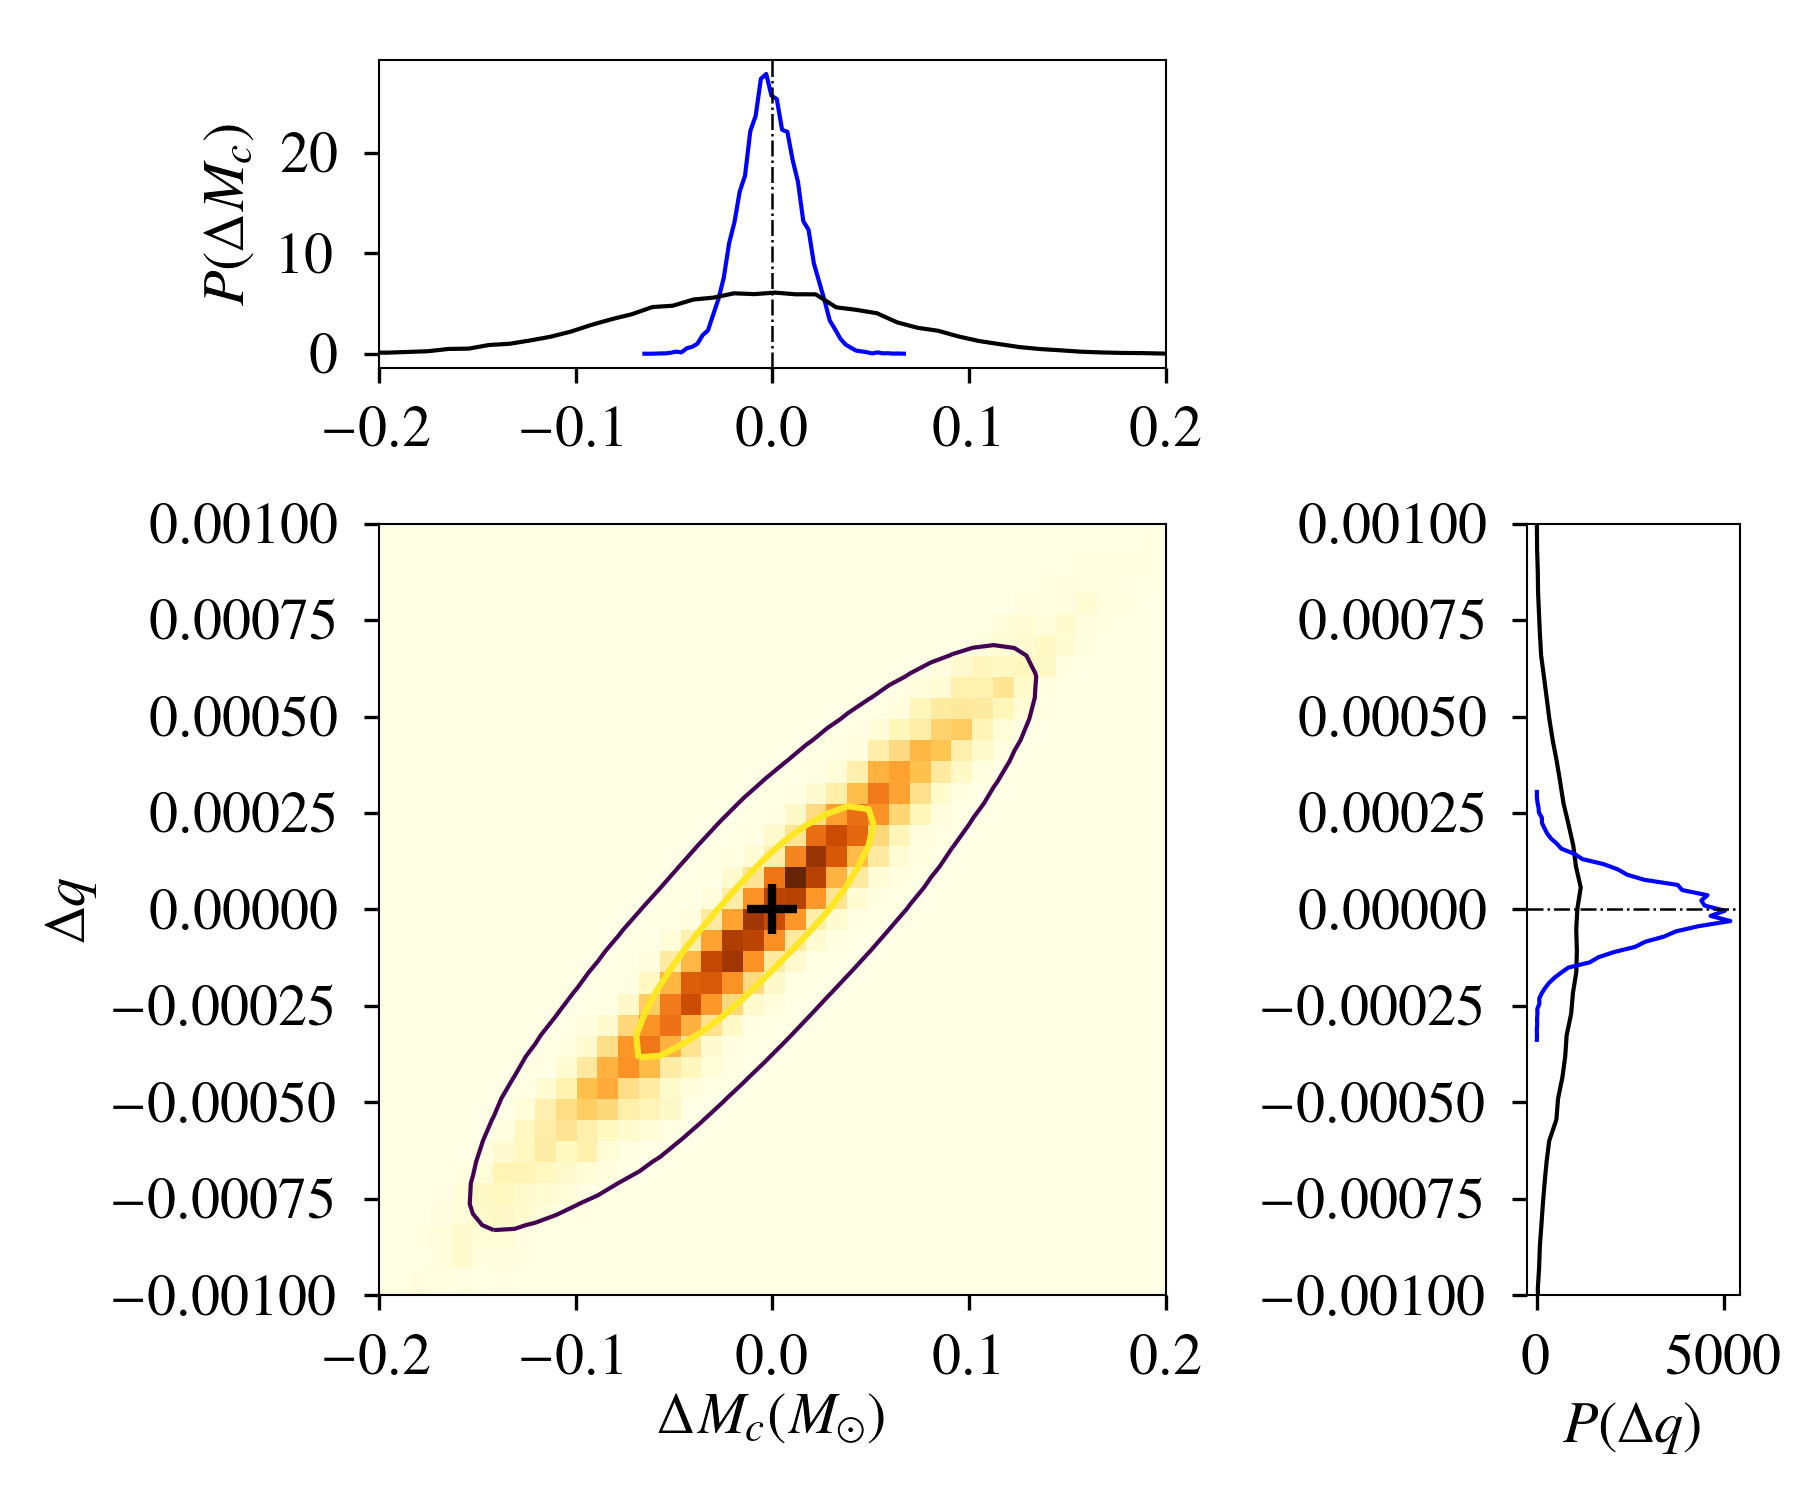
\includegraphics[width=3.4in]{figs/triangle_plot_gr.png}
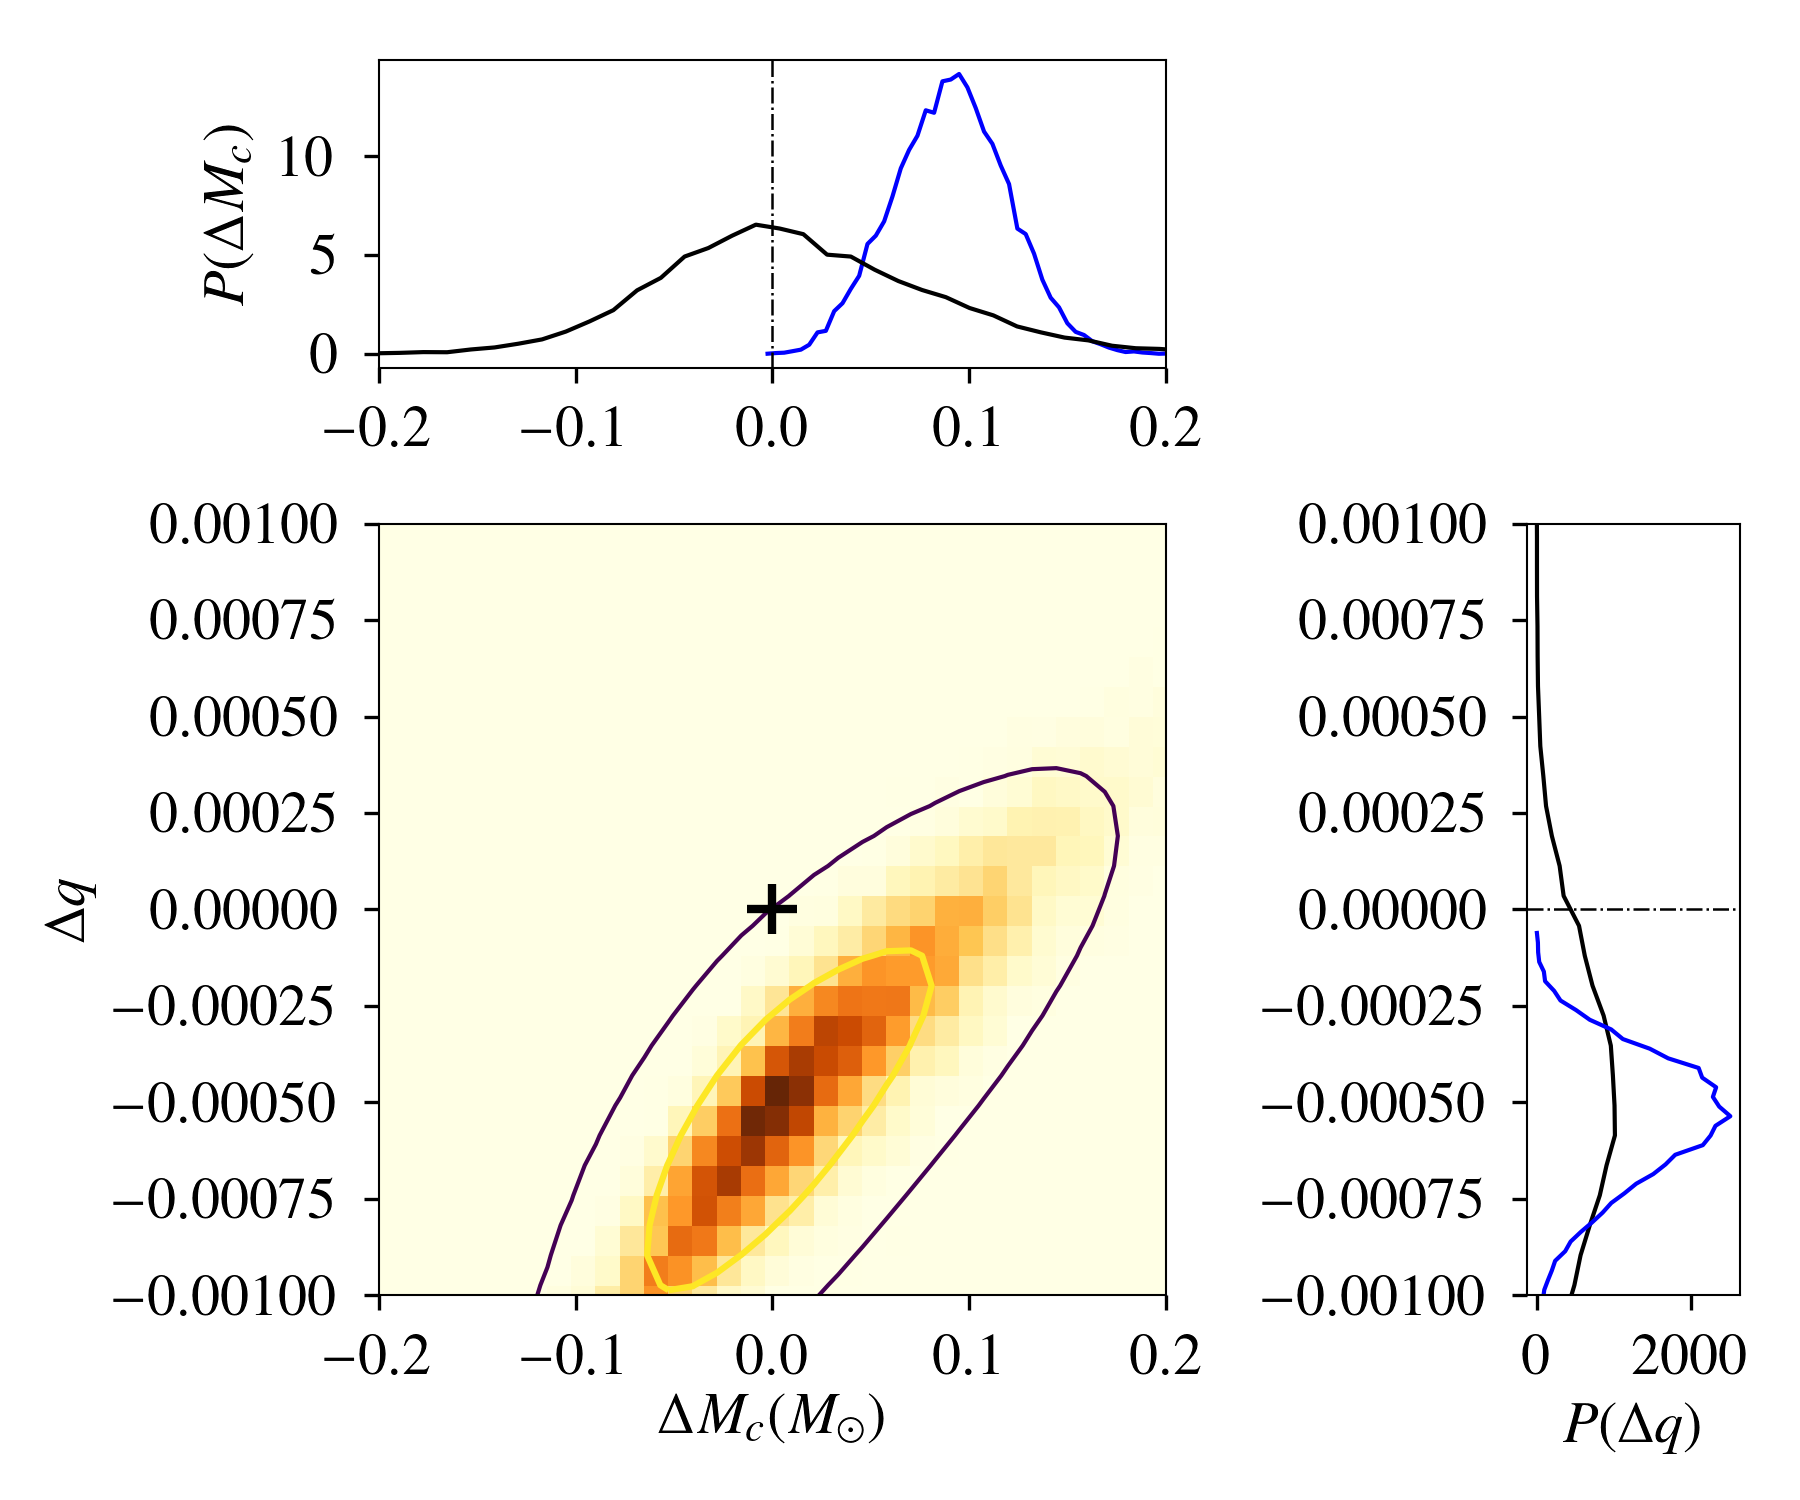
\includegraphics[width=3.4in]{figs/triangle_plot_mod_gr.png}
\caption{}
\label{fig:contour_plots}
\end{center} \end{figure*}
%%%%%%%%%%%%%%%%%%%%%%%%%%%%%%%%%%%%%%%%%%%%%%%%%%%%%%%%%%%%%%%%%%%%%%%%%%%%%%%%%%%%%%%%%%


\paragraph{Conclusions and future work:---}
%
%
\bibliographystyle{apsrev-nourl}
\bibliography{TGR_HM}

\end{document}
